\documentclass[12pt,oneside,a4paper]{book} % This style for A4 format.

%Packages
\usepackage{ecproject}
\usepackage{graphicx}
\usepackage{tikz}
\usetikzlibrary{calc}
\usepackage[a4paper, margin=1in]{geometry}
\usepackage{float}
\usepackage{qrcode}
%%%Page related
\usepackage{fancyhdr} % for header & footer
\usepackage[hidelinks]{hyperref}
\usepackage[acronym, toc, nonumberlist]{glossaries} %For Glossaries - to be loaded only after hyperref package

%\ifIndentPara
\usepackage{indentfirst}
%\fi
\usepackage{setspace}
%%%Table Related
%\usepackage{booktabs}
%\usepackage{makecell}
%\usepackage{multirow}
%\usepackage{multicol}


%Document settings
\title{Implementing Budget and Grant Analysis for Public Sector Management}
%%%%%%%%%%%%%%%Minor (or) Major report%%%%%%%%%%%%%%%
%Uncomment \MinorProject line, if the report is for Minor project.
\MinorProject
%%%%%%%%%%%%%%%%%%%%%%%%%%%%%%%%%%%%%%%%%%%%%%
%%%Student Details%%%
\stuNameA{Ayush Kumar}
\stuUSNA{1RV18IS009}
% \stuNameB{Nithin M}
% \stuUSNB{1RV16EC006}
% \stuNameC{Subrahmanya K N}
% \stuUSNC{1RV16EC007}
% \stuNameD{Subrahmanya K N}
% \stuUSND{1RV16EC007}

%%%Internal Guide%%%%
\guideNameA{Prof. Vanishree K}
\guideDesignationA{Assistant Professor}
\guideDeptA{Dept. of ISE}
\guideOrgA{RV College of Engineering}

%%%CoGuide%%%%
\guideNameB{Mohan George}
\guideDesignationB{Development Manager}
% \guideDeptB{SAP Labs India, Pvt Ltd}
\guideOrgB{SAP Labs India, Pvt Ltd}

%\guideNameC{Dr. Ramavenkateshwaran}
%\guideDesignationC{Assistant Professor}
%\guideDeptC{Dept. of ECE}
%\guideOrgC{RV College of Engineering}

\panelMemberA{__________}
\panelMemberDesigA{_________}
% \panelMemberB{Prof. P N Jayanthi}
% \panelMemberDesigB{Assistant Professor}

\Department[ISE]{Information Science and Engineering}

\HOD{Dr. B.M Sagar}
\Principal{Dr. K. N. Subramanya}

\academicYear{2021-2022}

\QRurl{}
\QRurl{https://www.google.com}
%%%%%%%%%%%%%%%%%%%For PG program%%%%%%%%%%%%%%%%%%%
%%%Uncomment \pgProgram command and define appropriate values for \MastersIn{} and \pgProgramName{}

%\pgProgram%
% \MastersIn[M.Tech]{Master of Technology}
% \pgProgramName{VLSI Design \& Embedded Systems}

%%%%%%%%%%%%%%%%%%Draft report%%%%%%%%%%%%%%%%%%
\DraftCopy
%%%%%%%%%%%%%%%%%%%%%%%%%%%%%%%%%%%%%%%%%%%%%%

%%%%%%%%%%%%%%%%%%Acronyms%%%%%%%%%%%%%%%%%%
\newglossary[sym]{symbolList}{sym1}{sym2}{List of Symbols}
% \newglossary[acr]{ac}{sym1}{sym2}{List of Symbols}
\makeglossaries
%Acronyms
\loadglsentries{./AuxFiles/Glossaries}
\renewcommand{\glspostdescription}{}% To remove dot at the end
%%%%%%%%%%%%%%%%%%%%%%%%%%%%%%%%%%%%%%%%%%%%%%

%%%%%%%%%%%%%%Bibliography%%%%%%%%%%%%%%%%%%%%%
\usepackage[backend=biber,style=ieee]{biblatex}
%If backend is set to bibtex, then configure texmaker Bi(La)Tex with "bibtex %"
\addbibresource{./AuxFiles/ProjectBib.bib}%Add bib file with extention
%%%%%%%%%%%%%%%%%%%%%%%%%%%%%%%%%%%%%%%%%%%%%%

%%%%%%%%%%%%%%%%WaterMark%%%%%%%%%%%%%%%%%%%%%
%%Use it only after Biblatex
\usepackage[printwatermark]{xwatermark}
\newwatermark[allpages,color=gray!50,angle=0,scale=2,xpos=0,ypos=0]{
\includegraphics[width=0.3\textwidth]{Figures/RVlogoVecW.png}}
% \usepackage{background}
% \backgroundsetup{scale=1, angle=0, firstpage = true, opacity=1, contents={
% \begin{tikzpicture}[remember picture, overlay]
% \node at ([yshift=0pt, xshift=0pt]current page.center){
\includegraphics[width=0.3\textwidth]{Figures/RV_logoVec.png}};
% \end{tikzpicture}
% }}
%%%%%%%%%%%%%%%%%%%%%%%%%%%%%%%%%%%%%%%%%%%%%%
\begin{document}
	\maketitle
	%\pagestyle{empty}
	\newpage
	\begin{spacing}{1.5}
		%%ecproject package is created by P Narashimaraja, Assistant Professor, ECE, RVCE
%Border
\begin{tikzpicture}[remember picture, overlay]
  \draw[line width = 4pt] ($(current page.north west) + (0.75in,-0.75in)$) rectangle ($(current page.south east) + (-0.75in,0.75in)$);
\end{tikzpicture}
\thispagestyle{empty}
% \vspace{-1cm}
\begin{center}
\Large\textbf{RV College of Engineering\textsuperscript{\small\textregistered}, Bengaluru} \par
\large{(\textit{Autonomous institution affiliated to VTU, Belagavi})} \par
\large\textbf{Department of \printDepartmentLF}\\
.\hspace{2cm}\\

\includegraphics[width=4cm]{Figures/RV_logoVec}\par
\Large\textbf{\underline{CERTIFICATE}} \par
\end{center}
%\begin{minipage}[b]{\linewidth}
%\large
\begin{spacing}{1.5}
\noindent Certified that the \ifMinor{minor\;}\else{ major\;}\fi project (18ISP81) work titled \textbf{\textit{\printTitle}} is carried out by
\ifPG{%
\textbf{\printStuNameA} (\textbf{\printStuUSNA}) who is  bonafide student 
}
\else{
\ifStuNameDUsed{%
\textbf{\printStuNameA } (\textbf{\printStuUSNA}), \textbf{\printStuNameB } (\textbf{\printStuUSNB}), \textbf{\printStuNameC } (\textbf{\printStuUSNC}) and \textbf{\printStuNameD } (\textbf{\printStuUSND})  who are bonafide students 
}\else{% 
\ifStuNameCUsed{%
\textbf{\printStuNameA } (\textbf{\printStuUSNA}), \textbf{\printStuNameB } (\textbf{\printStuUSNB}) and \textbf{\printStuNameC } (\textbf{\printStuUSNC})  who are bonafide students 
}\else{%
\ifStuNameBUsed{%
\textbf{\printStuNameA} (\textbf{\printStuUSNA}) and \textbf{\printStuNameB} (\textbf{\printStuUSNB})  who are bonafide students 
}\else{%
\textbf{\printStuNameA} (\textbf{\printStuUSNA}) who is  bonafide student 
}
\fi
}\fi
}\fi
}\fi
of RV College of Engineering, Bengaluru, in partial fulfillment of the requirements for the degree of  \ifPG \textbf{\printMastersInLF} in \textbf{\printMastersPrgName} \else\textbf{Bachelor of Engineering} in \textbf{\printDepartmentLF} \fi of the Visvesvaraya Technological University, Belagavi during the year \printAcadYear. It is certified that all corrections/suggestions indicated for the Internal Assessment have been incorporated in the \ifMinor{minor\;}\else{major\;}\fi project report deposited in the departmental library. The \ifMinor{minor\;}\else{ major\;}\fi project report has been approved as it satisfies the academic requirements in respect of \ifMinor{minor\;}\else{ major\;}\fi project work prescribed by the institution for the said degree.\\ \par
\end{spacing}

\begin{table}[H]
\centering
\resizebox{1\textwidth}{!}{%
\begin{tabular}{ccc}
\large Signature of Guide &\large Signature of Head of the Department &\large Signature of Principal\\
& &\\
\large\printGuideNameA & \large\printHOD & \large\printPrincipal\\
& & \\
\end{tabular}%
}
\end{table}

\begin{table}[H]
\centering
%\resizebox{\textwidth}{!}{%
\begin{tabular}{lccp{3cm}cc}
&&&\textbf{External Viva}&&\\
&&&&&\\
&Name of Examiners &&& & Signature with Date\\
% &&&&&\\
% 1.&&&&&\\
% &&&&&\\
% 2.&&&&&\\
\end{tabular}%
%}
\end{table}
%\pagebreak
		\newpage
		%%ecproject package is created by P Narashimaraja, Assistant Professor, ECE, RVCE
%%Border
\begin{tikzpicture}[remember picture, overlay]
  \draw[line width = 4pt] ($(current page.north west) + (0.75in,-0.75in)$) rectangle ($(current page.south east) + (-0.75in,0.75in)$);
\end{tikzpicture}

\thispagestyle{empty}

\begin{center}
  \Large\textbf{\underline{DECLARATION}} \par
\end{center}


\noindent \ifPG I \else \ifStuNameBUsed We\else I\fi\fi, \textbf{\printStuNameA}
\textbf{\printStuNameB} \ifStuNameCUsed  \ifStuNameDUsed ,$\,$ \else{$\,$ and $\,$}\fi 
\textbf{\printStuNameC}$\,$ \ifStuNameDUsed and $\,$ \textbf{\printStuNameD}$\,$ \fi \fi 
 students of \ifPG fourth \else \ifMinor{eighth\;}\else{eighth\;}\fi \fi semester 
 \ifPG \printMastersInSF\, in \printMastersPrgName \else B.E.\fi, Department of \printDepartmentLF,
  RV College of Engineering, Bengaluru, hereby declare that the \ifMinor{minor\;}\else{ major\;}\fi 
  project titled `\textbf{\printTitle}' has been carried out by \ifStuNameBUsed us \else me \fi and 
  submitted in partial fulfilment for the award of degree of \ifPG \textbf{\printMastersInLF} in 
  \textbf{\printMastersPrgName} \else\textbf{Bachelor of Engineering} in \textbf{\printDepartmentLF} 
  \fi during the year \printAcadYear.\\ \par
\noindent Further \ifPG I \else\ifStuNameBUsed we \else I \fi \fi 
declare that the content of the dissertation has not been submitted previously 
by anybody for the award of any degree or diploma to any other university.\\ \par

\noindent \ifPG I \else\ifStuNameBUsed We \else I \fi \fi also declare that any 
Intellectual Property Rights generated out of this project carried out at RVCE 
will be the property of RV College of Engineering, Bengaluru and we will be one 
of the authors of the same.

\vspace{1cm}
\noindent Place: Bengaluru\par
\vspace{0.5cm}
\noindent Date: \par

\vspace{2cm}
\begin{table}[H]
  \centering
  %\resizebox{\textwidth}{!}{%
  \begin{tabular}{llcp{5cm}cc}
       &                                &  &  &           & \\
       &                                &  &  &           & \\
       & Name                           &  &  & Signature & \\
       &                                &  &  &           & \\
    1. & \printStuNameA (\printStuUSNA) &  &  &           & \\
       &                                &  &  &           & \\
    \ifPG% 
    \else%
      \ifStuNameBUsed%
    2. & \printStuNameB (\printStuUSNB) &  &  &           & \\
       &                                &  &  &           & \\
      \else%
      \fi%
      \ifStuNameCUsed%
    3. & \printStuNameC (\printStuUSNC) &  &  &           & \\
       &                                &  &  &           & \\
      \else%
      \fi%
      \ifStuNameDUsed%
    4. & \printStuNameD (\printStuUSND) &  &  &           & \\
       &                                &  &  &           & \\
      \else%
      \fi%
    \fi%
  \end{tabular}%
  %}
\end{table}
%\pagebreak


		\newpage
		%%ecproject package is created by P Narashimaraja, Assistant Professor, ECE, RVCE.
%%Border
\begin{tikzpicture}[remember picture, overlay]
  \draw[line width = 4pt] ($(current page.north west) + (0.75in,-0.75in)$) rectangle ($(current page.south east) + (-0.75in,0.75in)$);
\end{tikzpicture}
\thispagestyle{empty}

\begin{center}
  %.\hspace{1cm}\\ \par
  \Large\textbf{\underline{ACKNOWLEDGEMENT}} \par
\end{center}

\ifPG I am \else
  \ifStuNameBUsed We are \else I am \fi\fi indebted to \ifPG my \else\ifStuNameBUsed
    our \else my \fi\fi guide, \textbf{Vanishree K} , Assistant Professor, \printGuideOrgA$\,$,
for her wholehearted support, suggestions and invaluable advice throughout this
Internship/Industrial training work and also helped in the preparation of this thesis.\\ \par

\ifPG I \else \ifStuNameBUsed We \else I \fi\fi also express my gratitude to \ifPG
  my \else\ifStuNameBUsed our \else my \fi\fi Manager \textbf{Mohan George},
Development Manager, SAP Labs India, Pvt Ltd, for his valuable comments and
suggestions during the phase evaluations. \\ \par

\ifPG My \else \ifStuNameBUsed Our \else My \fi\fi sincere thanks to \textbf{\printHOD},
Professor and Head, Department of \printDepartmentLF, RVCE for her support and encouragement.\\ \par


\ifPG I \else \ifStuNameBUsed We \else I \fi\fi express sincere gratitude to our beloved Principal, \textbf{\printPrincipal} for his appreciation towards this Internship/Industrial training work.\\ \par

\ifPG I \else\ifStuNameBUsed We \else I \fi\fi thank all the teaching staff and technical staff of the \printDepartmentLF\, department, RVCE for their help.\\ \par

Lastly, \ifPG I \else\ifStuNameBUsed we \else I \fi\fi take this opportunity to thank \ifPG my \else\ifStuNameBUsed our \else my \fi\fi family members and friends who provided all the backup support throughout the Internship training.\\ \par

%\pagebreak

\newpage
\begin{tikzpicture}[remember picture, overlay]
  \draw[line width = 4pt] ($(current page.north west) + (0.75in,-0.75in)$) rectangle ($(current page.south east) + (-0.75in,0.75in)$);
\end{tikzpicture}
\thispagestyle{empty}
\begin{center}
  %.\hspace{1cm}\\ \par
  \Large\textbf{\underline{Letter of Engagement}} \par

  \begin{figure}[H]
    \centering
    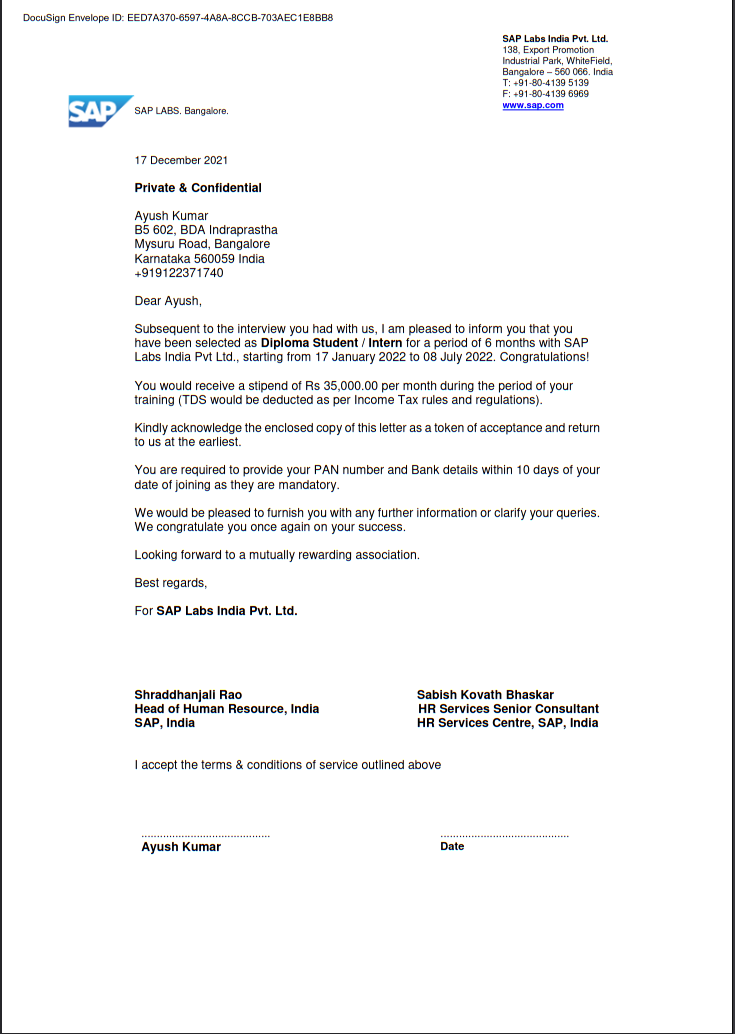
\includegraphics[scale=0.5]{Figures/internship_offer.png}
    \label{}
  \end{figure}
\end{center}
		\newpage
		\pagenumbering{roman}
		\chapter*{Abstract}
		\addcontentsline{toc}{chapter}{Abstract}\vspace{-1cm}
%Border
\begin{tikzpicture}[remember picture, overlay]
  \draw[line width = 4pt] ($(current page.north west) + (0.75in,-0.75in)$) rectangle ($(current page.south east) + (-0.75in,0.75in)$);
\end{tikzpicture}


\acrfull{sap} is an ERP (Enterprise Resource Planning) based software product company that supports and
manages business operations and customer relations of all types of companies, big to small scale.
SAP is a leading provider of cloud computing, enterprise mobility, and analytics to government and non-profit agencies worldwide. 

The SAP for Public Sector innovative solution portfolio to improve government performance, services, and accountability to improve people’s lives.
In the public sector, citizen engagement and service delivery operations are also becoming increasingly more complicated too. Government has a timeless mission to protect, provide, and prosper. Around the world, government organizations are trying to provide their citizens with economic opportunity, health care access, a sustainable environment, and better educational systems and infrastructure.

The frontend of the web application is built using SAP UI5 and SAP Fiori principles. The database
is configured on the in-memory, column-oriented SAP S/4 /acrshort{hana} Database, which helps in fast
retrieval and efficient storage of the data. Backend server-side coding is based on SAP Core \acrfull{abap}
(Advanced Business Application Programming Language), which is a 4th generation
programming language. Core Data Service Views are used for efficient data modelling. Frontend
and Backend services are connected via SAP OData and SAP Gateway.


\pagebreak
	\end{spacing}
	\newpage
	\pagestyle{fplain}
	\begin{spacing}{1.5}
		\tableofcontents
	\end{spacing}
	\newpage
	\begin{spacing}{1.5}
		\cleardoublepage
		\addcontentsline{toc}{chapter}{\listfigurename}
		\listoffigures
	\end{spacing}
	\newpage
	\begin{spacing}{1.5}
		\cleardoublepage
		\addcontentsline{toc}{chapter}{\listtablename}
		\listoftables
	\end{spacing}
	\newpage
	% \printglossary[type=\acronymtype,title=Acronyms]
	% \printglossary[type=symbolList, title= List of Symbols, toctitle=List of Symbols]

	\newpage
	\printglossary[type=\acronymtype, title= Abbreviations, toctitle=Abbreviations]


	\mainmatter
	\pagestyle{mplain}
	\glsresetall
	\newgeometry{top=2cm}
	\begin{spacing}{1.5}
		%Chapter 1 
		\chapter{Introduction}

\section[Introduction]{\textbf{Introduction}}
As society grows more complex, government faces a challenge and an opportunity. 
The challenge is to deliver on its mission to provide, protect, and prosper in 
an increasingly multifaceted society where it is difficult to develop one-size-fits-all 
programs that meet the precise needs of citizens

To deliver improved services to citizens,
governments at every level are faced with similar
set of challenges. One example is how to harness
the big data which has been acquired through
various touch points and other sources in order
to deliver impactful and relevant services along
with generating meaningful insights for intelligent
decision making.

As government delivers on its timeless mission to
provide for its citizens, protect them, and help
them prosper, it delivers services across a value
chain. That begins with reform, moves through
operations, delivers a service, measures
outcomes, and then begins again.

By adopting an artificial intelligence and machine
learning aligned data-driven strategy,
government can see the benefits of digital
transformation. Such a transformation can help
you to design innovative new business models. 
across multiple channels, optimize processes,
engage citizens and partners more effectively,
and manage change successfully. Armed with
360-degree insight, real-time recommendations,
and greater agility, you can better see the root
cause of problems, look for viable solutions, and
deploy them quickly. It can also help you to
report critical outcomes internally and externally,
reduce improper payments, and develop more
meaningful and impactful public policy. In short,
the transformation can help you function more
efficiently while increasing public trust and
support.


% You are allowed to use figures or diagrams which can help in introducing the topic acknowledging the source. For example , if you are introducing a particular topic, an appropriate figure can be used. The figure should be referenced in the text as Figure. \ref{fig:universe} 
\noindent\makebox[\textwidth]{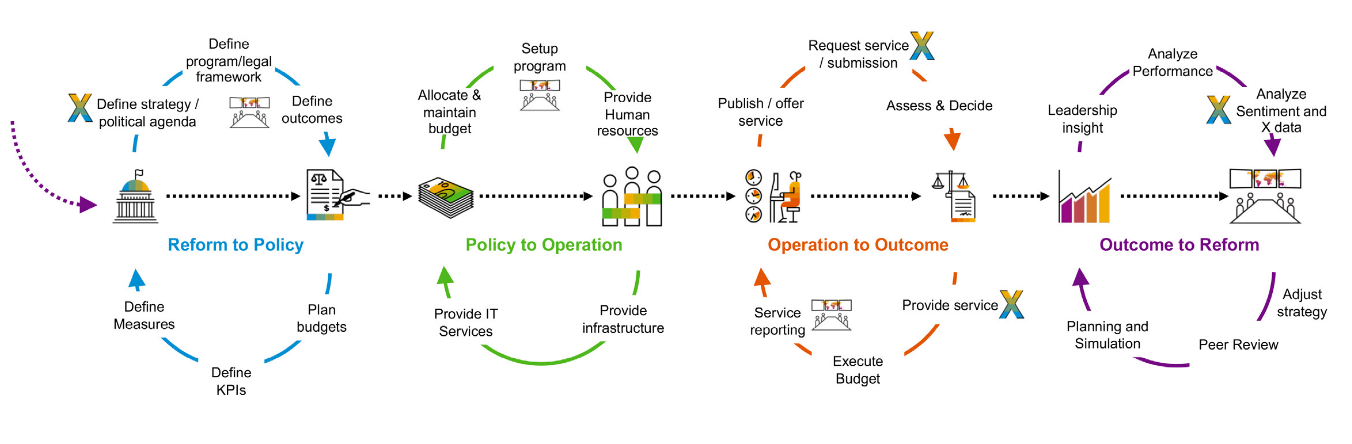
\includegraphics[width=\paperwidth]{Chapter1/Figures/img1.png}}
% \begin{figure}[htb]
% \centering
% 	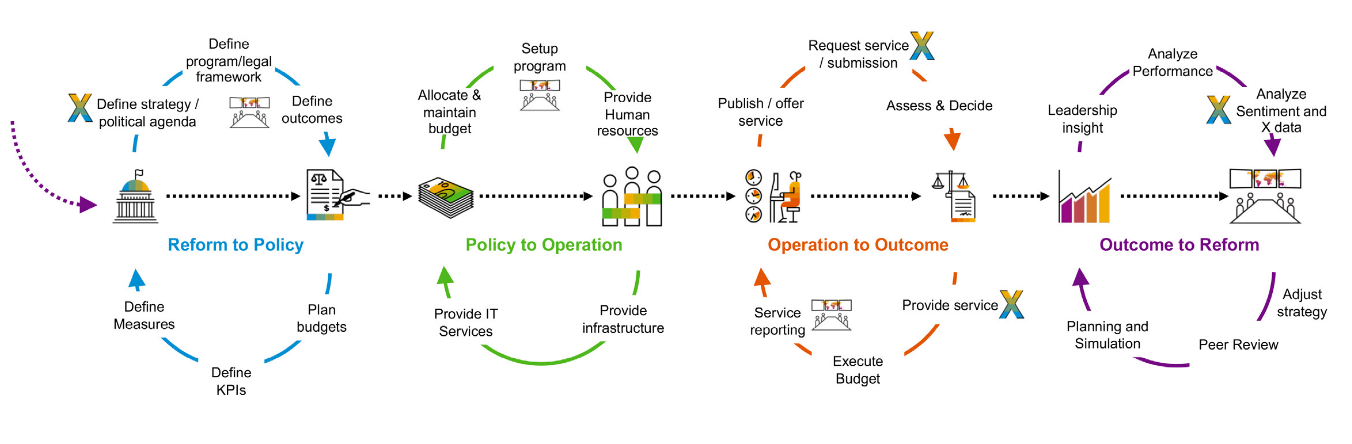
\includegraphics[width=\paperwidth]{Chapter1/Figures/img1.png}	
% 	\caption{Sample picture of universe }
% 	\label{fig:universe}
% \end{figure}

% These guidelines are provided to formally expose you to the various ethical and technical issues involved in writing up your work and the format you are required to adhere to while submitting your project report.

\section[Motivation]{\textbf{Motivation}}
The methods that government typically uses to
evaluate policies and outcomes may no longer be
sufficient to calibrate needed programs. As
complexity rises, the world is becoming more
interdisciplinary - problems can and do have
multiple root causes. The inability to approach
these root causes from multiple perspectives can
limit the efficacy of government action to solve
them.

However, most governments are not similarly managing
their data as a strategic asset to solve citizen problems,
meet citizen needs, and better understand the
consequences of potential new policies. Government
organizations still largely consider money, people,
facilities, and systems (not necessarily data) as their chief
assets. Very often data is perceived more as a problem
than a strategic asset.

% Brief the motivation of selecting your project title. You can elaborate the challenges in the specific area, relevance and importance of the chosen topic. 

\section[Problem statement]{\textbf{Problem statement}}

The core mission of the public sector – to protect the community, provide services,
and help the economy prosper – remains firmly in place. For public organizations,
success is measured not only by financial return on investment but even more so by
political and social return. Changes in technologies, citizen expectations, operational
models, and standards themselves require constant adaptation. Public sector
organizations must be able to respond to rapidly changing conditions and continue to
deliver outcomes within budget, yet still comply with standards

Designed to help all levels of government maximize public value, SAP for Public Sector solutions enable governments to optimize limited resources in public administration while delivering responsive front-office services. Our solutions support business processes across a wide range of government functions, from accounting and procurement to case management and social services.

SAP solutions help governments leverage their finite time, money, and personnel resources to fulfill mandated program and service requirements on a timely basis. Where two or more agencies share responsibility for a common outcome, these solutions can integrate information, processes, and technology to support the active collaboration that delivers financial returns, as well as social and political results, to internal and external government stakeholders. 

\section[Objectives]{\textbf{Objectives}}
This digital age is disruptive. Public sector organizations need strategic priorities that drive transformation. SAP envisions reimagined end-to-end (E2E)
business scenarios to support the strategic priorities of the digital economy.

The objectives of the project are
\begin{enumerate}
\item Put the citizen at the center

Continue your journey by further simplifying complicated
processes for the citizen, providing personalized, self-managed,
secure online engagement. Deliver the best customer experience
by connecting the front office to the back office. Become
anticipatory service orchestrators, information brokers, and
networkers.
\item Reimagine business processes and models

Lay a digital foundation for more efficient and agile processes,
to be able to quickly change when unforeseen disruptions
occur. Proactively adapt operational models and augment
everyday tasks so government workers can focus on the cases
that require human engagement.

\item Leverage data as an asset

Create a culture that is open and transparent – one that values
evidence over intuition and is based on an organization-wide
“single source of truth” that integrates interorganizational and
external data. Prioritize protection of data and privacy. Improve
services to citizens by adopting a data-driven strategy that
enables action from insight.

\item Enable the workforce of the future

Give employees every opportunity to do and be their best. Align
employee skills with organization needs, reduce compliance risk,
and keep remote workers engaged and productive. Track and
manage employee health and assess workforce engagement
and well-being. Understand potential implications for culture,
productivity, and the organization overall
\end{enumerate}

\section[Literature Review]{\textbf{Literature Review}}
% https://www.sap.com/documents/2017/01/a4303fdd-a07c-0010-82c7-eda71af511fa.html
% https://help.sap.com/doc/367477e6c8b94385bcd6404f06bc4c86/1.0.0.3/en-US/SBP_10FP03_Application_Help_en.pdf

% A literature review is a text of a scholarly paper, which includes the current knowledge including substantive findings, as well as theoretical and methodological contributions to a particular topic. Literature reviews are secondary sources, and do not report new or original experimental work. Most often associated with academic-oriented literature, such reviews are found in academic journals, and are not to be confused with book reviews that may also appear in the same publication. Literature reviews are a basis for research in nearly every academic field . A narrow-scope literature review may be included as part of a peer-reviewed journal article presenting new research, serving to situate the current study within the body of the relevant literature and to provide context for the reader. In such a case, the review usually precedes the methodology and results sections of the work.

\subsection{ERP Systems in Public Sector}

The vast majority of ERP system implementation in
production systems has been completed and consequently
the needs of that market have been satisfied. Some other
potential areas of ERP systems implementation were in
focus of ERP systems manufacturers. One of the emerging
markets is the public sector. Implementation of ERP
systems in the public sector has already began regardless
of some well-known ERP implementation problems such
as enormous investment and risk of failure in
implementation itself. Numerous published scientific
papers deal with various aspects of ERP systems, but the
number of papers regarding ERP systems implementation
in the public sector is relatively small. That particular area
of the public sector is becoming increasingly interesting for
ERP systems manufacturers, and researchers are interested
in the areas of public services where the ERP systems have
already been implemented. \cite*[]{Robert2014}

Following are the feilds where the ERP system can be systematically incorporated in Public sector 

\begin{table}[htb]
    \fontsize{10}{12}\selectfont
    \caption{Public Sector}
    \label{c1:tab1}
    \begin{center}
    \begin{tabular}{|p{3cm}|c|c|c|}
        %\hline
        %\multicolumn{4}{|c|}{Country List} \\
        \hline
        \textbf{Code }& \textbf {Non economic public sector} \\ \hline
        \textbf{PS1}    &   Education       \\\hline
        \textbf{PS2}    &   Culture         \\\hline
        \textbf{PS3}    &   Health careful  \\\hline
        \textbf{PS4}    &   Social Services \\\hline
        \textbf{PS5}    &   Law Enforcement \\\hline
        \textbf{PS6}    &   Military – defense\\\hline
        \textbf{PS7}    &   Public library   \\\hline
    \end{tabular}
    \end{center}
    \end{table}
    


\subsection{Available ERP Solutions}

\subsubsection*{Aptean}

Aptean was founded in 2012 after a merger between Consola Corporation and CDC Software and currently offers ERP solutions for several financial and manufacturing markets. The company builds and acquires solutions to support the evolving operational needs of businesses. Aptean’s ERP solutions include Cimnet ERP, Encomprix ERP, Ross ERP, and more, each designed to fit individual needs. Aptean delivers solutions to global customers in the manufacturing, distribution, high tech, transportation, retail, government, real estate, financial services, health care, and not-for-profit industries. \cite{Budget2019}


\subsubsection*{Deltek}

Deltek’s ERP solution, Costpoint, has assisted companies in researching and identifying new opportunities, winning new business, recruiting and developing talent, and more. Deltek offers a range of ERP products to fit the unique demands of clients. Deltek’s ERP solutions are available as cloud-based and on-premise systems, priced per employee per month. Deltek is typically used by organizations with over 21 employees and more than ten users who need the software. The solution is used in several industries, including aerospace and defense, healthcare, non-profits, and education.  \cite{Nizar2021}


\subsubsection*{Infor}
Infor is a privately held software company founded in 2002. Infor’s business applications are specialized by industry, built for the cloud, and gives you everything you need to run your day-to-day operations as well as grow your business for the long term. Whether you need to optimize vital back-office functions like HR and financials, jumpstart your customer experience, or initiate digital transformation, Infor solutions have you covered. Over 90,000 organizations worldwide rely on Infor to help overcome market disruptions and achieve business-wide digital transformation.
\cite{Rachel2022}


\subsubsection*{Microsoft}
Microsoft provides ERP software to businesses of all sizes through its Dynamics 365 platform, consisting of six products: Microsoft AX, GP, SL, NAV, CRM, RMS. The Microsoft Dynamics portfolio started in 2001 with the acquisition of Great Plains Software and Soloman and in 2002 with the acquisition of Navison and Axapta. Together, these four technologies make up the Microsoft Business Solutions Group (MBS), a major supplier of ERP solutions. Dynamics GP, NAV, and SL are typically intended for small and medium enterprises, while Dynamics AX is best suited for larger organizations.

\cite{Robert2014}


\subsubsection*{Oracle NetSuite}
For more than 20 years, Oracle NetSuite has helped organizations grow, scale, and adapt to change. NetSuite provides a suite of cloud-based applications, including financials / ERP, HR, professional services automation, and omnichannel commerce, used by more than 15,000 customers in 203 countries and dependent territories. ERP software from Oracle NetSuite allows consolidation in real-time and includes automated intercompany eliminations and foreign currency translation. The solution is web-based and runs on a range of Internet browsers. The company ensures safety by using its built-in security controls and data center.

\cite{Thompson2019}


\subsubsection*{OpenGov}
OpenGov provides cloud ERP solutions for public sector budgeting, community development, and financial management. Over 1,000 governments across the U.S. rely on OpenGov to help allocate resources, increase efficiency, improve public engagement, and make data and information readily available to staff and elected officials. The OpenGov ERP Cloud offers four main products: Budgeting and Planning; Financials; Reporting and Transparency; Permitting, Licensing and Code Enforcement.
\cite{Vasyl2021}

\subsubsection*{SAP}
SAP, the German software giant, provides businesses with its SAP S/4HANA next-generation ERP software that provides strong functionality across many industries, including manufacturing, services, retail, wholesale distribution, and more. S/4HANA offers applications covering customer relationship management, financials, human capital management, and product lifecycle management. The software primarily serves small to medium-sized businesses with one hundred employees and less than 75 million USD in annual revenue.


\subsubsection*{Tyler Technologies}

Tyler Technologies’ solutions help governments and schools better serve their communities with technology designed to simplify complex processes. This vendor’s broad solutions and product offering empower you to deliver better and faster assistance to the public — greater transparency and accessibility, sustainable office practices, secure data that’s easy to manage and maintain, and faster results. Tyler Technologies offers various solutions geared toward public administration, courts and public safety, health, human services, and K-12 education.

\subsubsection*{Unanet}
Unanet for Government Contractors makes managing GovCon projects easy, providing perfect clarity and total control over day-to-day operations, forecasting, and planning. Purpose-built in-house by GovCon professionals, Unanet features support DCAA requirements at each stage. This vendor also integrations PSA and PPM with Financials to help organizations reliably plan, track, and manage projects and people. Unanet also offers ERP for professional services and A/E.

% \ref{fig:ERPmillitary} 
\begin{figure}[htb]
\centering
	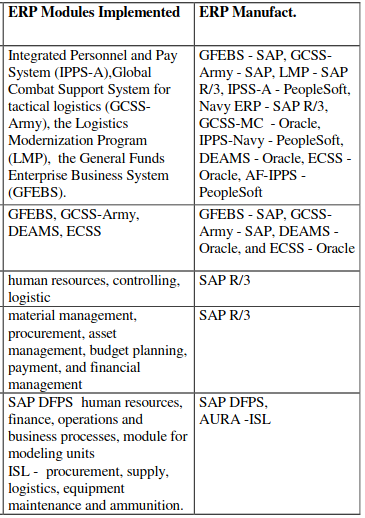
\includegraphics[scale=0.5]{Chapter1/Figures/ERP3.png}	
	\caption{ERP system used in millitary sector} 
	\label{fig:ERPmillitary}
\end{figure}

% \ref{fig:ERPEducation} 
\begin{figure}[htb]
\centering
	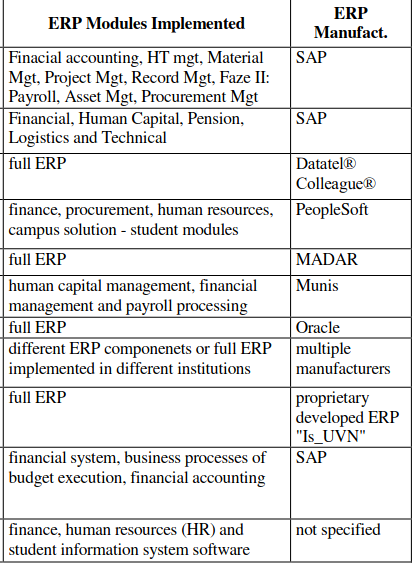
\includegraphics[scale=0.5]{Chapter1/Figures/ERP1.png}	
	\caption{ERP system used in education sector}
	\label{fig:ERPEducation}
\end{figure}

% \ref{fig:ERPFinance} 
\begin{figure}[htb]
\centering
	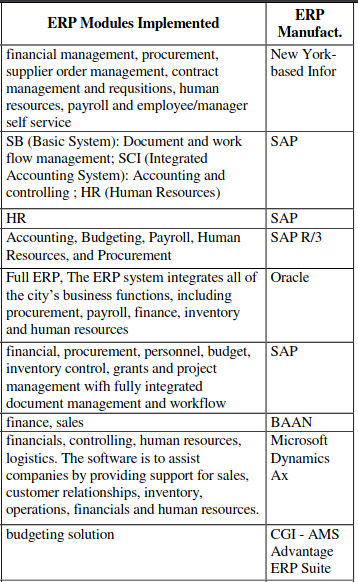
\includegraphics[scale=0.5]{Chapter1/Figures/ERP2.png}	
	\caption{ERP system used in financial sector }
	\label{fig:ERPFinance}
\end{figure}

% \ref{fig:ERPHealthcare} 
\begin{figure}[htb]
    \centering
        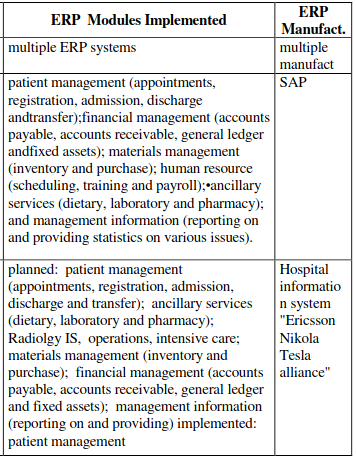
\includegraphics[scale=0.5]{Chapter1/Figures/ERP4.png}	
        \caption{ERP system used in healthcare sector }
        \label{fig:ERPHealthcare}
    \end{figure}
    





    
% \subsubsection[Review types]{\textbf{Review types}}

% The main types of literature reviews are: evaluative, exploratory, and instrumental. A fourth type, the systematic review, is often classified separately, but is essentially a literature review focused on a research question, trying to identify, appraise, select and synthesize all high-quality research evidence and arguments relevant to that question. A meta-analysis is typically a systematic review using statistical methods to effectively combine the data used on all selected studies to produce a more reliable result.


% \subsubsection[Process and product]{\textbf{Process and product}}

% Distinguish between the process of reviewing the literature and a finished work or product known as a literature review. The process of reviewing the literature is often ongoing and informs many aspects of the empirical research project. All of the latest literature should inform a research project. Scholars need to be scanning the literature long after a formal literature review product appears to be completed.

% \subsubsection{\textbf{Page limitation}}

% A careful literature review is usually 15 to 30 pages and could be longer. The process of reviewing the literature requires different kinds of activities and ways of thinking and link the activities of doing a literature review with Benjamin Bloom’s revised taxonomy of the cognitive domain (ways of thinking: remembering, understanding, applying, analysing, evaluating, and creating).

% This section should contain the review of the literature in the past.You should review a minimum of 10 papers from standard reference journals. Kindly avoid local conference papers and papers from predatory journals. Kindly consult with your guide and finalize papers to be considered for review before adding in this section.Report the major observations and findings from each paper in one paragraph in the format given below.

%  proposed various techniques for adders and multipliers.Add the reference papers to the bibliography section using Jabref and cite it here using the instructions given in further chapters.


% \subsubsection{\textbf{Plagiarism}}

% To use someone else's exact words without quotation marks and appropriate credit, or to use the unique ideas of someone else without acknowledgement, is known as plagiarism. In publishing, plagiarism is illegal; in other circumstances, it is, at the least, unethical. You may quote or paraphrase the words or ideas of another if you document your source. Although you need not enclose the paraphrased material in quotation marks, you must document the source. 

% Paraphrased ideas are taken from someone else whether or not the words are identical. Paraphrasing a passage without citing the source is permissible only when the information paraphrased is common knowledge in a field. (Common knowledge refers to historical, scientific, geographical, technical, and other type of information on a topic readily available in handbooks, manuals, atlases and other references). 

% \subsubsection{How to add Reference}
% Use \texttt{Jabref} which will help in adding the reference in a separate file, from which one can use \verb|\citep\{\}| command to add reference. A sample, referring to a textbook would look something like this,\cite{Razavi2000}.

% \cite{Budget2019}
% \cite{Nizar2021}
% \cite{Rachel2022}
% \cite{Robert2014}
% \cite{Thompson2019}
% \cite{Vasyl2021}

% \section[Brief Methodology of the project]{\textbf{Brief Methodology of the project}}
% Discuss about the methodology you identified to execute the objectives of your project in brief. Methodology is a system of practices, techniques, procedures, and rules used to execute a particular project. You can elaborate the methodology in a later chapter. Here you can present in the form of a flow diagram and explain the methodology in a paragraph.

% \section[Assumptions made / Constraints of the project]{\textbf{Assumptions made / Constraints of the project}}

% List the assumptions made for the execution of the project in this section. You can also elaborate on the major constraints of the project. This section should clearly state under what conditions your project is valid. It is mandatory to have this section in your project report.

% \section[Organization of the report]{\textbf{Organization of the report}}

% This report is organized as follows. Write the discussions in each chapter. A sample is as follows.
% \begin{itemize}
% \item Chapter 2 discusses the fundamentals of ADC and the performance parameters for evaluation.
% \item Chapter 3 discusses .
% \item Chapter 4 discusses .
% \item Chapter 5 discusses .
% \item Chapter 6 discusses .
% \end{itemize}

.

		%Chapter 2
		\chapter{Requirement specification}

From Chapter 2 onwards, every chapter should start with an introduction paragraph. This paragraph should brief about the flow of the chapter. This introduction can be limited within 4 to 5 sentences. The chapter heading should be appropriately modified (a sample heading is shown for this chapter).But don't start the introduction paragraph in the chapters 2 to end with "This chapter deals with....". Instead you should bring in the highlights of the chapter in the introduction paragraph.

\section{Contents of this chapter}

This chapter should discuss about the prerequisite learnings before the execution of the project. Organise and elaborate the theory and necessary fundamentals required for the execution of the project. You can use \verb|\subsections| and \verb|subsubsections| in this chapter.
\section{Contents of this chapter}
If a specific programming language is required for the project, a section can be allotted in this chapter to discuss it. 
\section{Contents of this chapter}
Tools used could be another possible section to discuss about the software tools used in the work. 
\section{Contents of this chapter}
The details in this chapter can be added in consultation with the project guide. For an internship based projects, subsections can be modified accordingly. 

\section{Use of Acronyms and Glossaries}
Acronyms are nothing but the short form of regular repeated word. Say for example, you have a repeat word "Integrated Circuits" and you want to use a short form for it as "IC". For which you have to first define the word and use it wherever you wanted to refer it.

First, let's look at the definition, which has to be entered in \texttt{Glossaries.tex} under \texttt{CoverPages} directory.
\begin{verbatim}
%\newacronym{<Ref>}{<Short-Form>}{<Expanded word>}
\newacronym{ic}{IC}{Integrated Circuits}
\end{verbatim}
In order to use the defined acronym, use the commands \verb|\gls{<Ref>}| as shown below

As an example, call the definition with \verb|\gls{ic}| and the outcome of it is reflected as, \gls{ic}.

Note: For the First time, the expanded form appears along with the Short-form definition inside parenthesis. But when the \verb|\gls{}| is repeated, only Short-form appears inside the parenthesis.

Now, let's look at the definition of symbols. Follow the syntax to define the symbol first, inside \texttt{Glossaries.tex} under \texttt{CoverPages} directory.
\begin{verbatim}
%\newglossaryentry{<Ref>}{name=<Symbol>, description={<description about the symbol>}, type=<List type>}
\newglossaryentry{rc}{name=$\tau$, description={Time constant}, type=symbolList}
\end{verbatim}

As an example, the rate of change is defined with \verb|\gls{rc}| and the outcome of it is reflected as, the rate of change is defined with \gls{rc}.

\vspace{0.75cm}

 \textbf{The chapters should not end with figures, instead bring the paragraph explaining about the figure at the end followed by a summary paragraph.}

After elaborating the various sections of the chapter (From Chapter 2 onwards), a summary paragraph should be written discussing the highlights of that particular chapter. This summary paragraph should not be numbered separately. This paragraph should connect the present chapter to the next chapter.


		%Chapter 3
		% \chapter{Design}

\indent\indent From Chapter 2 onwards, every chapter should start with an introduction paragraph. This paragraph should brief about the flow of the chapter. This introduction can be limited within 4 to 5 sentences. The chapter heading should be appropriately modified (a sample heading is shown for this chapter).But don't start the introduction paragraph in the chapters 2 to end with "This chapter deals with....". Instead you should bring in the highlights of the chapter in the introduction paragraph. 
\section{Contents of this Chapter}
This chapter should contain the following sections and subsections in detail.
\begin{enumerate}
\item Specifications for the Design
\item Pre analysis work for the design or Models used
\item Design methodology in detail
\item Design Equations
\item Experimental techniques (if any)
\end{enumerate}
Apart from the aforementioned sections, you can add sections as per the requirements of the project in consultation with your guide.

\section{Paraphrasing}
When you paraphrase a written passage, you rewrite it to state the essential ideas in your own words. Because you do not quote your source word for word when paraphrasing, it is unnecessary to enclose the paraphrased material in quotation marks. However, the paraphrased material must be properly referenced because the ideas are taken from someone else whether or not the words are identical. 

Ordinarily, the majority of the notes you take during the research phase of writing your report will paraphrase the original material. Paraphrase only the essential ideas. Strive to put original ideas into your own words without distorting them."

\section{Quotations}
When you have borrowed words, facts, or idea of any kind from someone else's work, acknowledge your debt by giving your source credit in footnote (or in running text as cited reference). Otherwise, you will be guilty of plagiarism. Also, be sure you have represented the original material honestly and accurately. Direct word to word quotations are enclosed in quotation marks."

\vspace{0.75cm}

 \textbf{The chapters should not end with figures, instead bring the paragraph explaining about the figure at the end followed by a summary paragraph.}

After elaborating the various sections of the chapter (From Chapter 2 onwards), a summary paragraph should be written discussing the highlights of that particular chapter. This summary paragraph should not be numbered separately. This paragraph should connect the present chapter to the next chapter.  

		%Chapter 4
		% \chapter{Implementation Detail}

\indent\indent From Chapter 2 onwards, every chapter should start with an introduction paragraph. This paragraph should brief about the flow of the chapter. This introduction can be limited within 4 to 5 sentences. The chapter heading should be appropriately modified (a sample heading is shown for this chapter).But don't start the introduction paragraph in the chapters 2 to end with "This chapter deals with....". Instead you should bring in the highlights of the chapter in the introduction paragraph. 

\section{Contents of this chapter}
This chapter should elaborate the following in detail.
\begin{enumerate}
\item Implementation details for hardware based projects
\item Top level Design for software based projects
\end{enumerate}

You can add sections and sub sections to elaborate your project work done.

\vspace{0.75cm}

 \textbf{The chapters should not end with figures, instead bring the paragraph explaining about the figure at the end followed by a summary paragraph.}

After elaborating the various sections of the chapter (From Chapter 2 onwards), a summary paragraph should be written discussing the highlights of that particular chapter. This summary paragraph should not be numbered separately. This paragraph should connect the present chapter to the next chapter. 



		% Chapter 5
		% \chapter{Results \& Analysis}
\indent\indent From Chapter 2 onwards, every chapter should start with an introduction paragraph. This paragraph should brief about the flow of the chapter. This introduction can be limited within 4 to 5 sentences. The chapter heading should be appropriately modified (a sample heading is shown for this chapter).But don't start the introduction paragraph in the chapters 2 to end with "This chapter deals with....". Instead you should bring in the highlights of the chapter in the introduction paragraph.
\section{Contents of this chapter}
All the results obtained for your objectives should be discussed in this chapter. This chapter should contain the following sections as per the project.
\begin{enumerate}
\item Simulation results
\item Experimental results
\item Performance Comparison
\item Inferences drawn from the results obtained
\end{enumerate}
All the figures should be properly explained by bringing the scenarios of the design done in the project. A detailed discussion of results obtained should be done in this chapter.

\section{Tables in thesis}
\begin{itemize}
	\item All Table Caption should be in Sentence Case, TNR 10 Pt. It should be of the Format:
	\begin{itemize}
		\item Table 1.1 Results of the experiment ….(Centered)
	\end{itemize}
	\item It should be cited as Table 1.1.
	\item Caption should appear above the Table.
	\item Table Header and the entries should be of Font TNR 10 Pt, Justified.
	\item For wider Table, the page orientation can be Landscape.
	\item For Larger Table, it can run to pages and the header should be repeated for each page of the Table.
	\item Table must be adjusted to fit in the page and no single row is left out for a new page.	
\end{itemize}

Sample Table \ref{c5:tab1} and Table \ref{c5:tab2} are given below  for your reference,

\begin{table}[htb]
\fontsize{10}{12}\selectfont
\caption{Country List}
\label{c5:tab1}
\begin{tabular}{|p{3cm}|c|c|c|}
	%\hline
	%\multicolumn{4}{|c|}{Country List} \\
	\hline
	\textbf{Country Name     or Area Name}& \textbf {ISO ALPHA 2 Code} & \textbf {ISO ALPHA 3 Code} & \textbf{ISO numeric Code}\\
	\hline
	\textbf{Afghanistan}   & AF    & AFG &   004\\\hline
	\textbf{Aland Islands}&   AX  & ALA   & 248\\\hline
	\textbf{Albania} & AL & ALB&  008\\\hline
	\textbf{Algeria}    &DZ & DZA&  012\\\hline
	\textbf{American Samoa}&   AS  & ASM&016\\\hline
	\textbf{Andorra}& AD  & AND   & 020\\\hline
	\textbf{Angola}& AO  & AGO& 024\\
	\hline
\end{tabular}
\end{table}

%\begin{table}[htp]
%\fontsize{10}{12}\selectfont
%\centering
%\caption{Data units, sources, and dates} \label{c5:tab2}
%\begin{tabular}{| *4{>{\arraybackslash}m{1in}|} @{}m{0pt}@{}}
%	\hline
%	\textbf{Variable} & \textbf{Dates} & \textbf{Units} &
%	\textbf{Source}  &\\[2ex] 
%	\hline
%	\textbf{Nominal Physical Capital Stock} & 1950-1990 & Billions
%			US\$ & Nehru and Dhareshwar (1993) &\\[0ex]
%	\hline
%	\textbf{Total Population} & 1950-1990 & Billions & Nehru and
%			Dhareshwar (1993) &\\[0ex]
%	\hline
%	\textbf{Nominal GDP} & 1950-1990 & Billions  US\$ & PWT &\\[5ex]
%	\hline
%	\textbf{Real GDP per capita} & 1950-1990 & 2005 US\$ per capita & PWT &\\[5ex]
%	\hline
%\end{tabular}
%\end{table}

\section{Math equation in thesis}
All equation should be written using equation editor or using an equivalent tool.
\begin{itemize}
	\item Equations should be numbered as : 1.1, 1.2 ...
	\item Equation should be Centered, 12 Pt, TNR. 
	\item Equation number should be right Justified
	\item It should be cited as Eqn. 1.1.
   \item If the sentence starts by citing an equation, then it should be written as Equation 1.1 For example, Equation 5.1 states the Pythagoras theorem.

	
\end{itemize}

For example in Eqn. \ref{c5:eqn1}, The well known Pythagorean theorem $x^2 + y^2 = z^2$ was 
proved to be invalid for other exponents. 
Meaning the next equation has no integer solutions:

\begin{equation}
\label{c5:eqn1}
	x^n + y^n = z^n
\end{equation}

The mass-energy equivalence is described by the famous equation in Eqn. \ref{c5:eqn2}
\begin{equation}
\label{c5:eqn2}
	E=mc^2
\end{equation}

discovered in 1905 by Albert Einstein. 

\vspace{0.75cm}

 \textbf{The chapters should not end with figures, instead bring the paragraph explaining about the figure at the end followed by a summary paragraph.}

After elaborating the various sections of the chapter (From Chapter 2 onwards), a summary paragraph should be written discussing the highlights of that particular chapter. This summary paragraph should not be numbered separately. This paragraph should connect the present chapter to the next chapter.





		%Chapter 6
		% \chapter{Conclusion}

\section{Conclusion}
This chapter should not contain an introduction paragraph like other chapters. You can directly write conclusion of the work done under this section. Typically this section can have 3 to 4 paragraphs. 

First paragraph should bring in the scenario of the project and every objective should be explained here.

Second paragraph should say how the objectives are implemented and achieved.

Last paragraph should draw the conclusions from each objective with quantitative results, performance improvement etc. 

\section{Future Scope}
Briefly discuss the constraints and limitations of the project and state the possibilities of extending the work in future.
\section{Learning Outcomes of the Project}
\begin{itemize}
\item List the learning outcomes here
\item List a minimum of 5 learning outcomes
\end{itemize}


		
		\backmatter
		\clearpage
		%\ifDrft{
		%%Do Nothing
		%}\else{
		\printbibliography%
		%}
		%\printindex
	\end{spacing}
\end{document}